\documentclass[11pt,a4paper]{article}

% === Font & encoding (XeLaTeX) ===
\usepackage{fontspec}
\setmainfont{Latin Modern Roman}
\setsansfont{Latin Modern Sans}
\setmonofont{Latin Modern Mono}

% Korean font support via ucharclasses
\usepackage{ucharclasses}
\newfontfamily\koreanfont{Droid Sans Fallback}[Scale=0.95]
\setTransitionsForCJK{\koreanfont}{\setmainfont{Latin Modern Roman}}

% === Layout ===
\usepackage[margin=2cm,headheight=14pt]{geometry}
\usepackage{graphicx}
\usepackage{booktabs}
\usepackage{longtable}
\usepackage{float}
\usepackage{hyperref}
\usepackage{xcolor}
\usepackage{fancyhdr}
\usepackage{titlesec}
\usepackage{caption}
\usepackage{multirow}
\usepackage{enumitem}
\usepackage{array}
\usepackage{tabularx}
\usepackage{amssymb}
\usepackage[normalem]{ulem}

% === Header/Footer ===
\pagestyle{fancy}
\fancyhf{}
\rhead{Cross-Model SAE Analysis}
\lhead{LLM Gambling Addiction}
\cfoot{\thepage}

% === Section styling ===
\titleformat{\section}{\Large\bfseries}{\thesection}{1em}{}
\titleformat{\subsection}{\large\bfseries}{\thesubsection}{1em}{}
\titleformat{\subsubsection}{\normalsize\bfseries}{\thesubsubsection}{1em}{}

% === Hyperlinks ===
\hypersetup{
    colorlinks=true,
    linkcolor=blue!60!black,
    citecolor=green!50!black,
    urlcolor=blue!70!black
}

% === Title ===
\title{\textbf{Cross-Model, Cross-Domain Neural Basis of\\Risky Decision-Making in LLMs}\\[0.3em]
\normalsize ``Can Large Language Models Develop Gambling Addiction?''}
\author{Seungpil Lee, Donghyeon Shin, Yunjeong Lee, Sundong Kim\\
\small GIST (Gwangju Institute of Science and Technology)}
\date{March 22, 2026}

\begin{document}
\maketitle
\tableofcontents
\newpage

% ============================================================
% OVERVIEW
% ============================================================
\section*{Overview}
\addcontentsline{toc}{section}{Overview}

When a large language model goes bankrupt in a gambling task---repeatedly choosing to bet until its balance reaches zero---what happens inside the network? This report asks whether that internal ``bankruptcy signal'' is a universal property shared across different models, gambling domains, and experimental conditions, or whether each setting produces its own distinct neural pattern.

Two transformer models are analyzed: \textbf{Gemma-2-9B-IT} (Google, 42 layers, 3{,}584-dim) and \textbf{LLaMA-3.1-8B-Instruct} (Meta, 32 layers, 4{,}096-dim). Each plays three negative-expected-value gambling paradigms---Investment Choice (IC), Slot Machine (SM), and Mystery Wheel (MW)---totaling 16{,}000 games across 6 model--paradigm combinations. Betting conditions (Fixed/Variable) and prompt components (Goal, Money, Warning, Hint, Persona) are systematically varied.

Internal representations are examined at two levels. \textbf{Hidden states} capture the full activation vector at each transformer layer. \textbf{SAE features} are sparse, interpretable decompositions of those hidden states, extracted via GemmaScope (131K features/layer) and LlamaScope (32K features/layer). Classification uses StandardScaler $\rightarrow$ PCA(50) $\rightarrow$ Logistic Regression (balanced, $C$=1.0) with 5-fold stratified cross-validation. Transfer AUC with 200-permutation tests provides statistical significance.

\textbf{Three research questions}:
\begin{itemize}[nosep]
    \item \textbf{RQ1}: Do Gemma and LLaMA share common bankruptcy (BK) patterns?
    \item \textbf{RQ2}: Do BK patterns persist when the gambling domain changes?
    \item \textbf{RQ3}: Do BK patterns persist when betting conditions change?
\end{itemize}

\bigskip\hrule\bigskip

% ============================================================
% EXECUTIVE SUMMARY
% ============================================================
\section*{Executive Summary}
\addcontentsline{toc}{section}{Executive Summary}

\textbf{RQ1---Both models encode bankruptcy with near-identical accuracy and balanced neural structure.} Gemma and LLaMA achieve BK classification AUC within 0.006 of each other in every paradigm (0.954--0.976). At L22, Gemma has 600 and LLaMA has 1{,}334 universal BK neurons, both with approximately equal promoting and inhibiting counts. After controlling for bet-type and paradigm, 65--76\% of SAE features remain BK-significant (permutation $p$=0.000 vs ${\sim}$1\% null).

\textbf{RQ2---BK classifiers trained in one domain predict bankruptcy in another.} Gemma IC$\rightarrow$MW transfer reaches AUC 0.932 (L18); LLaMA MW$\rightarrow$IC reaches 0.805 (L25). Both models achieve this despite near-orthogonal per-paradigm weight vectors (cosine $\approx$ 0.04), indicating BK signal occupies a shared low-dimensional subspace rather than a single direction.

\textbf{RQ3---A classifier trained on Fixed-bet bankruptcies predicts Variable-bet bankruptcies, and vice versa.} Cross-bet-type transfer yields AUC 0.74--0.93 across all LLaMA layers (all $p$=0.000). Gemma SAE confirms the pattern at deep layers (L30: 0.902). 415 SAE features show consistent BK effects (same sign, $d$$\geq$0.3) under both betting conditions.

\bigskip\hrule\bigskip

% ============================================================
% 1. SETUP
% ============================================================
\section{Setup}

\subsection{Data}

\begin{table}[H]
\centering
\caption{Dataset Overview}
\begin{tabular}{llccc}
\toprule
\textbf{Paradigm} & \textbf{Model} & \textbf{Games} & \textbf{BK} & \textbf{BK\%} \\
\midrule
IC & Gemma & 1{,}600 & 172 & 10.8\% \\
IC & LLaMA & 1{,}600 & 142 & 8.9\% \\
SM & Gemma & 3{,}200 & 87 & 2.7\% \\
SM & LLaMA & 3{,}200 & 1{,}164 & 36.4\% \\
MW & Gemma & 3{,}200 & 54 & 1.7\% \\
MW & LLaMA & 3{,}200 & 2{,}426 & 75.8\% \\
\bottomrule
\end{tabular}
\end{table}

Each paradigm uses 2 bet types (Fixed/Variable) and 32 prompt combinations. IC additionally varies bet constraints (c10/c30/c50/c70). LLaMA's BK rates are 13--44$\times$ higher than Gemma's in SM and MW, meaning the two models adopt very different behavioral strategies while encoding BK information with equivalent accuracy (see \S\ref{sec:rq1_classification}).

\subsection{Key Definitions}

\begin{description}[style=nextline, leftmargin=2em]
    \item[Bankruptcy (BK)] Balance reaches \$0 through accumulated losses. The primary outcome variable.
    \item[Decision Point (DP)] The model's activation state at its final bet-or-stop decision in each game.
    \item[Universal BK neuron] A neuron whose correlation with BK outcome is FDR-significant (BH, $p$<0.01) in every paradigm tested, with the same sign.
    \item[Cross-domain transfer] Train a BK classifier on one paradigm, test on another. AUC $\gg$ 0.5 with permutation $p$<0.05 indicates shared BK structure.
    \item[Cross-bet-type transfer (F1)] Train a BK classifier on Fixed-bet games, test on Variable-bet games (and vice versa).
\end{description}

\bigskip\hrule\bigskip

% ============================================================
% 2. RQ1
% ============================================================
\section{RQ1: Do Both Models Share Common BK Patterns?}

\subsection{BK Classification}\label{sec:rq1_classification}

Both models achieve BK classification AUC > 0.95 in all three paradigms at their respective best layers.

\begin{table}[H]
\centering
\caption{BK Classification AUC}
\begin{tabular}{lccc}
\toprule
\textbf{Paradigm} & \textbf{Gemma} & \textbf{LLaMA} & \textbf{Difference} \\
\midrule
SM & 0.976 (L20) & 0.974 (L8) & 0.002 \\
IC & 0.960 (L30) & 0.954 (L12) & 0.006 \\
MW & 0.966 (L30) & 0.963 (L16) & 0.003 \\
\bottomrule
\end{tabular}
\end{table}

The two models peak at different depths---Gemma at L20--L30, LLaMA at L8--L16---but their best AUC values differ by at most 0.006. This holds even though LLaMA MW's BK rate (75.8\%) is 44$\times$ higher than Gemma MW (1.7\%). The classification pipeline uses balanced class weights, so this equivalence is not an artifact of base rate. BK information is present in both architectures at comparable fidelity.

\subsection{Universal BK Neurons}

\begin{table}[H]
\centering
\caption{Universal BK Neurons (L22)}
\begin{tabular}{lcc}
\toprule
 & \textbf{Gemma (3-paradigm)} & \textbf{LLaMA (2-paradigm)} \\
\midrule
Total neurons & 3{,}584 & 4{,}096 \\
Universal BK neurons & 600 (16.7\%) & 1{,}334 (32.6\%) \\
Promoting / Inhibiting & 302 / 298 & 672 / 662 \\
\bottomrule
\end{tabular}
\end{table}

LLaMA's higher count primarily reflects the different chance levels: 2-paradigm sign-consistency has a 50\% chance baseline vs 25\% for 3-paradigm. The key finding is not the absolute count but the \textbf{balanced ratio}: both models encode BK through roughly equal numbers of promoting and inhibiting neurons at every layer tested (L8--L30). This bidirectional structure suggests a ``push-pull'' mechanism where BK-promoting and BK-inhibiting signals coexist.

\subsection{Factor Decomposition}

For each SAE feature, OLS regression (\texttt{feature $\sim$ outcome + bet\_type + paradigm}) tests whether BK outcome contributes independently after controlling for bet-type and paradigm.

\begin{table}[H]
\centering
\caption{Outcome-Significant Features}
\begin{tabular}{lcccc}
\toprule
\textbf{Model} & \textbf{Paradigms} & \textbf{Features} & \textbf{Outcome-Significant} & \textbf{Permutation Null} \\
\midrule
Gemma & IC+SM+MW & 581 & 65.2\% (379) & ${\sim}$1\% \\
LLaMA & IC+SM & 1{,}418 & 69.5\% (985) & ${\sim}$1\% \\
LLaMA & IC+SM+MW & 1{,}056 & 75.8\% (800) & ${\sim}$1\% \\
\bottomrule
\end{tabular}
\end{table}

Within LLaMA, adding MW as a third paradigm increases the outcome-significant proportion from 69.5\% to 75.8\%, indicating that additional domains filter out paradigm-specific noise without diluting the BK signal. All three decompositions exceed the permutation null (${\sim}$1\%) by 60$\times$+.

\begin{figure}[H]
\centering
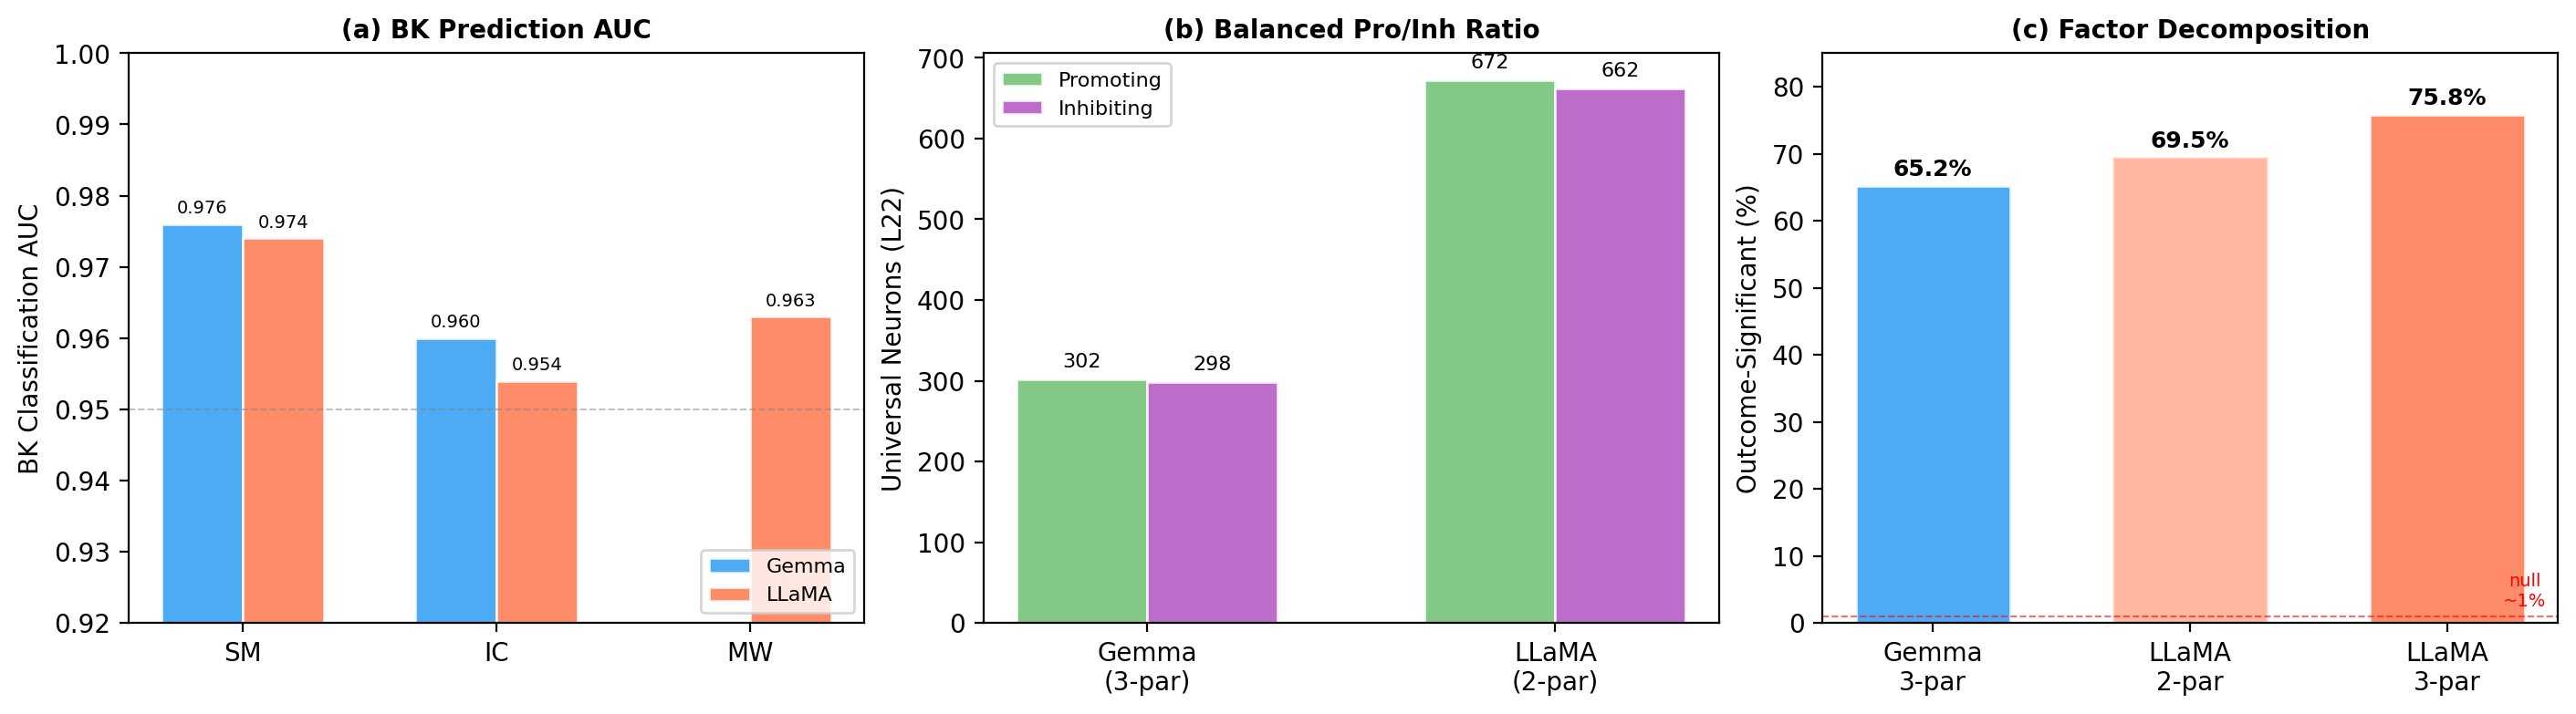
\includegraphics[width=\textwidth]{figures/v10_fig1_rq1_overview.png}
\caption{(a) Cross-model BK classification AUC. (b) Universal BK neurons: balanced promoting/inhibiting ratio. (c) Factor decomposition: 65--76\% outcome-significant vs ${\sim}$1\% null.}
\label{fig:rq1_overview}
\end{figure}

\subsection{RQ1 Summary}

BK prediction accuracy is equivalent across architectures (AUC difference $\leq$ 0.006). Both models maintain a balanced promoting/inhibiting neuron structure. 65--76\% of SAE features encode BK independently of confounds. These three observations are consistent with a shared BK representation that arises in both architectures despite different training data and model sizes.

\bigskip\hrule\bigskip

% ============================================================
% 3. RQ2
% ============================================================
\section{RQ2: Does the BK Pattern Persist Across Domains?}

\subsection{Cross-Domain Transfer}

\begin{table}[H]
\centering
\caption{Gemma SAE Transfer (Best Layer)}
\begin{tabular}{lcc}
\toprule
\textbf{Transfer} & \textbf{AUC} & \textbf{$p$} \\
\midrule
IC $\rightarrow$ MW & 0.932 & 0.000 \\
IC $\rightarrow$ SM & 0.913 & 0.000 \\
SM $\rightarrow$ MW & 0.867 & 0.000 \\
MW $\rightarrow$ IC & 0.853 & 0.000 \\
SM $\rightarrow$ IC & 0.646 & 0.000 \\
\bottomrule
\end{tabular}
\end{table}

\begin{table}[H]
\centering
\caption{LLaMA 3-Paradigm Transfer (Best Layer)}
\begin{tabular}{lcc}
\toprule
\textbf{Transfer} & \textbf{AUC} & \textbf{$p$} \\
\midrule
MW $\rightarrow$ IC & 0.805 & 0.000 \\
SM $\rightarrow$ IC & 0.749 & 0.000 \\
IC $\rightarrow$ MW & 0.680 & 0.000 \\
MW $\rightarrow$ SM & 0.682 & 0.000 \\
IC $\rightarrow$ SM & 0.577 & 0.000 \\
\bottomrule
\end{tabular}
\end{table}

Both models show strong transfer involving MW (AUC 0.68--0.93), while IC$\leftrightarrow$SM transfer is weaker and layer-dependent. MW serves as a ``hub'' paradigm: BK patterns learned from or applied to MW transfer well to other domains.

\begin{figure}[H]
\centering
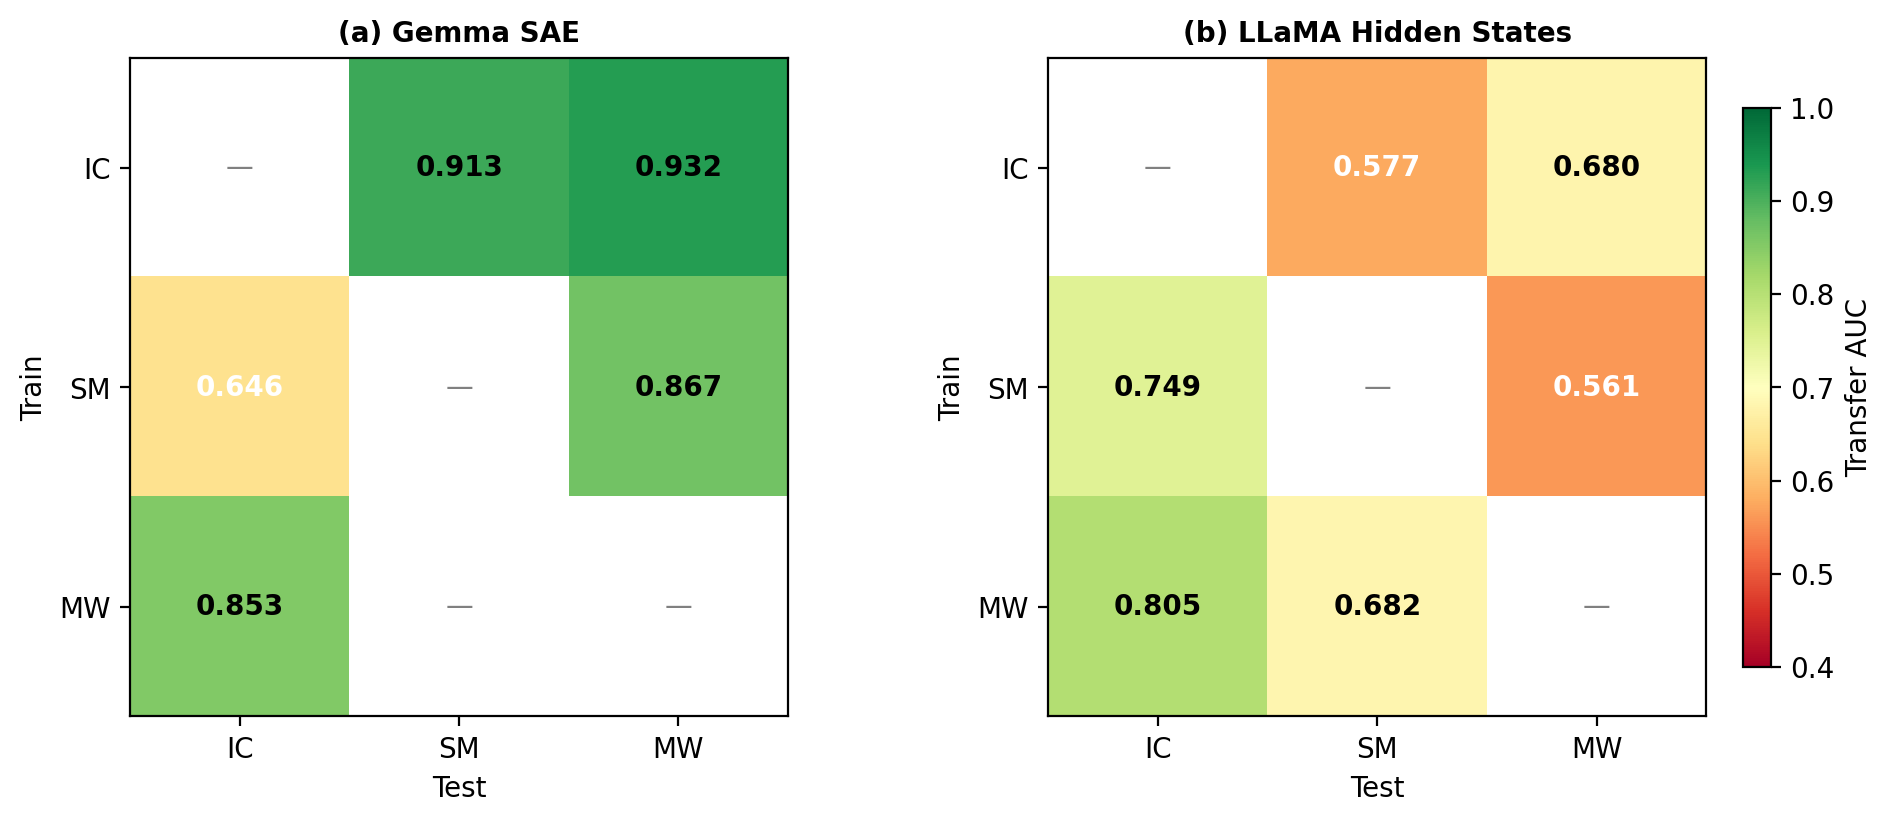
\includegraphics[width=\textwidth]{figures/v10_fig2_rq2_transfer.png}
\caption{Cross-domain transfer heatmaps. (a) Gemma SAE. (b) LLaMA hidden states. Green = high transfer; yellow/red = weak.}
\label{fig:rq2_transfer}
\end{figure}

\subsection{Shared BK Subspace}

Per-paradigm classifiers produce weight vectors that are nearly orthogonal (cosine $\approx$ 0.04), yet a low-dimensional subspace extracted via PCA on these weight vectors achieves high AUC.

\begin{table}[H]
\centering
\caption{Shared Subspace Performance}
\begin{tabular}{lcc}
\toprule
 & \textbf{Gemma (3D)} & \textbf{LLaMA (2D)} \\
\midrule
IC AUC & 0.862 & 0.901 \\
SM AUC & 0.899 & 0.943 \\
MW AUC & 0.970 & --- \\
Weight cosine & ${\sim}$0.04 & 0.038 \\
\bottomrule
\end{tabular}
\end{table}

Near-orthogonal weight vectors with high subspace AUC means BK signal is distributed across a multi-dimensional subspace rather than concentrated along a single axis.

\subsection{Hidden States vs SAE in Transfer}

Hidden states outperform SAE in most cross-domain transfer directions (Gemma IC$\rightarrow$SM: +0.247; SM$\rightarrow$MW: +0.101; LLaMA SM$\rightarrow$IC: +0.064). SAE sparsification can lose cross-domain coherence, suggesting that BK signal relies partly on distributed, low-magnitude activations that sparse decomposition discards.

\subsection{RQ2 Summary}

Cross-domain transfer succeeds in both models (AUC 0.58--0.93, all $p$=0.000), with MW as the strongest hub paradigm. A shared low-dimensional subspace captures BK despite orthogonal weight vectors. BK encoding generalizes across gambling domains at deep layers.

\bigskip\hrule\bigskip

% ============================================================
% 4. RQ3
% ============================================================
\section{RQ3: Does the BK Pattern Persist Across Betting Conditions?}

\subsection{Cross-Bet-Type Transfer (F1)}

A BK classifier trained exclusively on Fixed-bet games is applied to Variable-bet games, and vice versa.

\begin{table}[H]
\centering
\caption{LLaMA IC Hidden State Transfer}
\begin{tabular}{lccc}
\toprule
\textbf{Layer} & \textbf{Fix$\rightarrow$Var AUC} & \textbf{Var$\rightarrow$Fix AUC} & \textbf{Both $p$} \\
\midrule
L8 & 0.872 & 0.842 & 0.000 \\
L12 & 0.772 & 0.927 & 0.000 \\
L22 & 0.736 & 0.912 & 0.000 \\
L30 & 0.819 & 0.911 & 0.000 \\
\bottomrule
\end{tabular}
\end{table}

\begin{table}[H]
\centering
\caption{Gemma IC SAE Transfer}
\begin{tabular}{lccc}
\toprule
\textbf{Layer} & \textbf{Fix$\rightarrow$Var AUC} & \textbf{Var$\rightarrow$Fix AUC} & \textbf{Both $p$} \\
\midrule
L18 & 0.808 & 0.726 & 0.000 \\
L30 & 0.902 & 0.696 & 0.000 \\
L10 & NS & NS & --- \\
\bottomrule
\end{tabular}
\end{table}

In LLaMA, every layer and both directions yield $p$=0.000. Var$\rightarrow$Fix transfer (0.84--0.93) is consistently stronger than Fix$\rightarrow$Var (0.74--0.87), possibly because Variable games explore a wider activation space that encompasses the Fixed BK region. In Gemma, deep layers succeed (L30: Fix$\rightarrow$Var 0.902) while the shallow layer (L10) fails---consistent with the general pattern that cross-condition transfer requires deep representations. Note that Gemma IC has only 14 Variable BK cases, limiting statistical power for Gemma-specific bet-type analyses.

\begin{figure}[H]
\centering
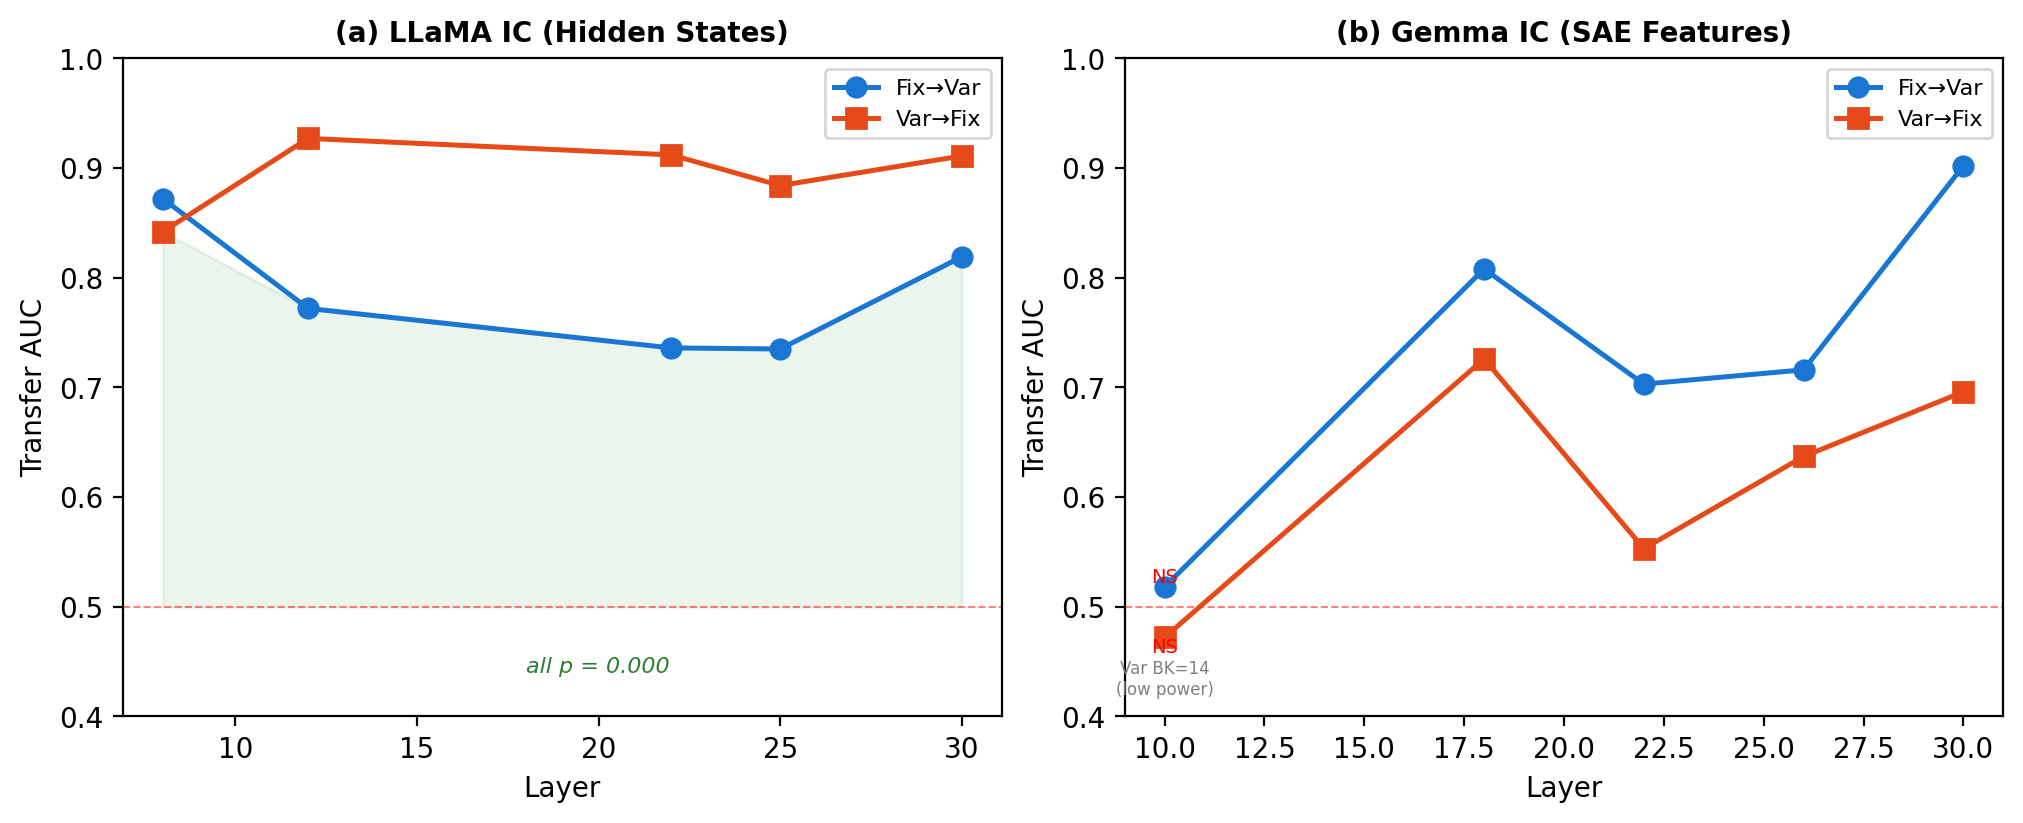
\includegraphics[width=\textwidth]{figures/v10_fig3_rq3_bettype_transfer.png}
\caption{Cross-bet-type transfer. (a) LLaMA: all layers, both directions, all $p$=0.000. (b) Gemma SAE: deep layers succeed; L10 fails.}
\label{fig:rq3_bettype}
\end{figure}

\subsection{Direction Cosine and Common Features}

The cosine similarity between Variable BK direction and Fixed BK direction provides complementary evidence. LLaMA IC shows $\cos > 0.81$ at all hidden state layers and $\cos$ 0.77--0.85 at SAE level. Gemma IC converges from negative at shallow layers to $\cos$ ${\sim}$0.39 at L30---weaker due to the Variable BK sample size ($n$=14).

At SAE L22, 415 LLaMA features (and 35 Gemma features) show $d$$\geq$0.3 in both betting conditions with the same sign. The balanced promoting/inhibiting ratio (LLaMA: 213/202) mirrors the universal neuron structure from \S2.2.

\begin{figure}[H]
\centering
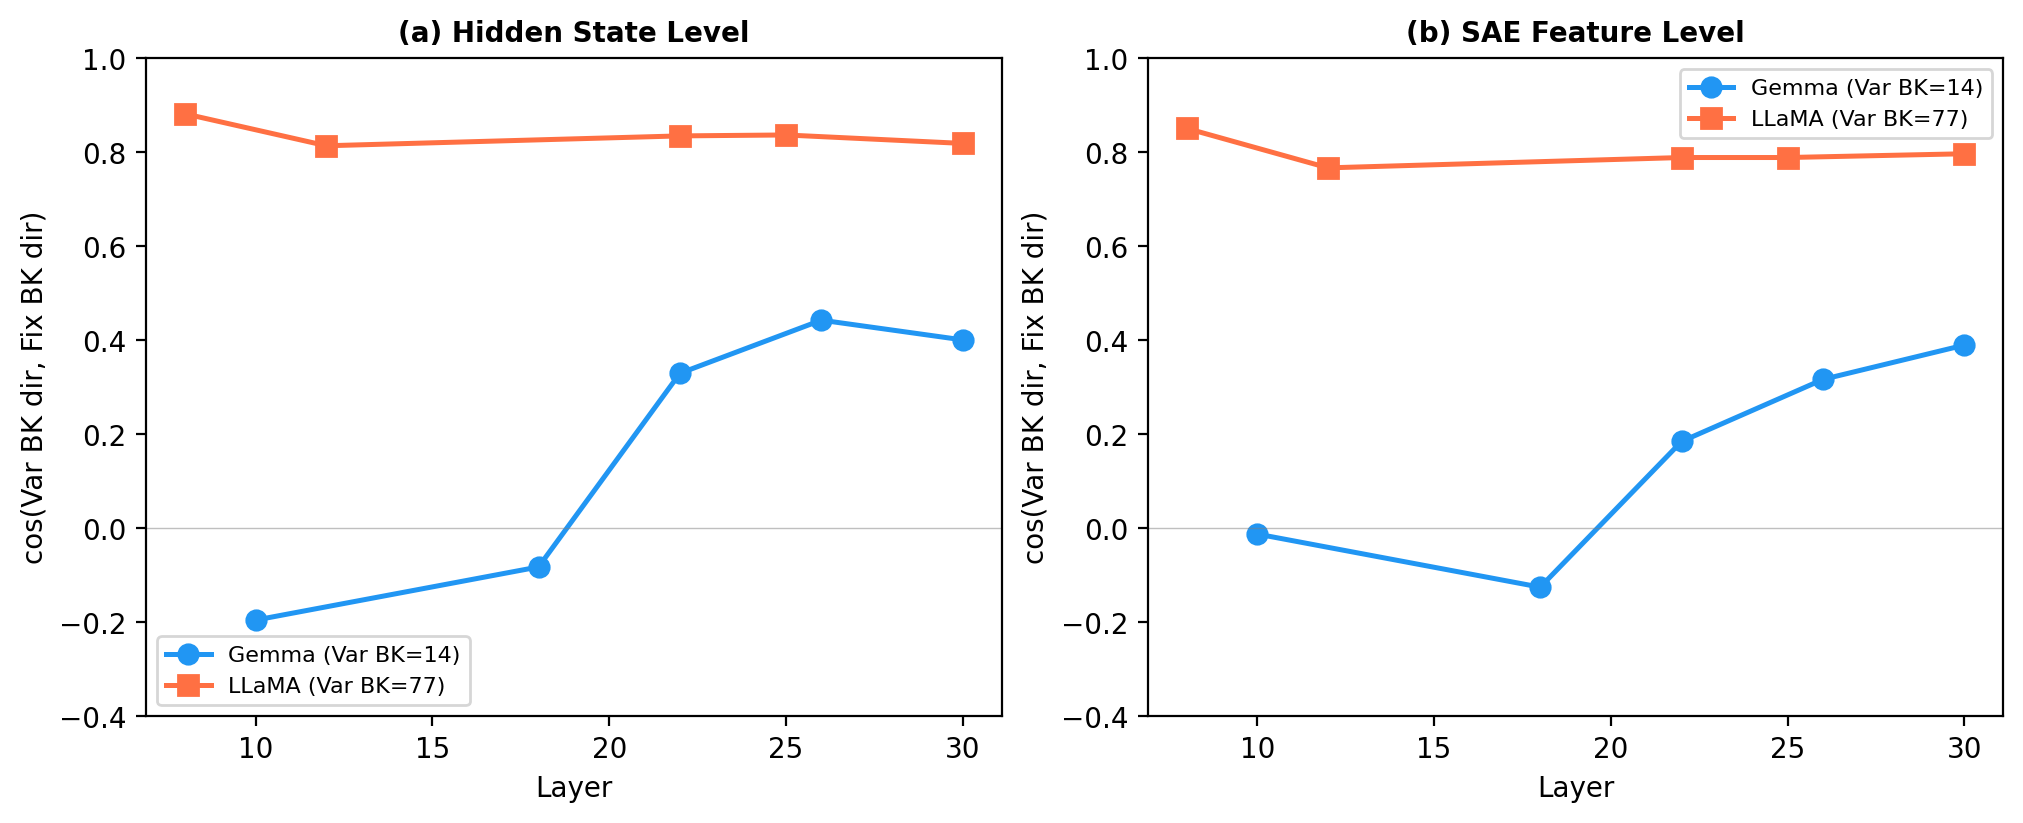
\includegraphics[width=\textwidth]{figures/v10_fig4_rq3_direction_cosine.png}
\caption{Var/Fix direction cosine at (a) hidden state and (b) SAE level. LLaMA $\cos$>0.77 at all layers; Gemma converges at deep layers.}
\label{fig:rq3_cosine}
\end{figure}

\subsection{G-Prompt and Bet Constraint Effects}

The G (Goal-setting) prompt shifts activations toward the BK direction in both models ($\cos$ = +0.85 in Gemma SM, +0.63 in LLaMA SM at L22). Bet constraints (c10$\rightarrow$c70) map linearly onto BK probability (Gemma $r$=0.979, LLaMA $r$=0.987; note $n$=4 data points limits the strength of this linear claim). These observations suggest that the BK representation encodes continuous risk magnitude rather than a binary BK/Safe distinction.

\subsection{RQ3 Summary}

The F1 cross-bet-type transfer analysis provides direct evidence that Fixed and Variable betting conditions share the same underlying BK representation at deep layers. Direction cosines, common features, and G-prompt alignment all point in the same direction. BK encoding is robust to the Fixed/Variable manipulation in both models.

\bigskip\hrule\bigskip

% ============================================================
% 5. IMPLICATIONS
% ============================================================
\section{Implications for NMT Paper \S3.2}

The paper's \S3.2 identifies 112 causal features in LLaMA SM via activation patching, with safe features in L4--L19 and risky features in L24+. This analysis extends that single-model, single-domain finding in three ways:

\textbf{Cross-model}: Gemma achieves near-identical BK classification (0.976 vs 0.974) and exhibits the same balanced promoting/inhibiting neuron structure. The 112 causal features likely reflect a property present in both architectures, not a LLaMA-specific artifact.

\textbf{Cross-domain}: BK classifiers transfer across IC, SM, and MW with AUC up to 0.932. Factor decomposition shows 65--76\% of features encode BK independently of paradigm. The causal features identified in SM likely generalize to other gambling domains.

\textbf{Cross-condition}: Cross-bet-type transfer (AUC 0.74--0.93) demonstrates that BK representations are robust to the Fixed/Variable manipulation---the same manipulation that produces the paper's central behavioral finding (Variable betting increases bankruptcy). The neural representation remains stable even as behavioral outcomes diverge.

\bigskip\hrule\bigskip

% ============================================================
% 6. LIMITATIONS
% ============================================================
\section{Limitations}

\begin{enumerate}[leftmargin=2em]
    \item \textbf{Correlational evidence only.} All analyses in this report are correlational. Causal validation via activation patching has been performed only in LLaMA SM (paper \S3.2). Cross-model and cross-domain causal validation remains pending.

    \item \textbf{Sample size imbalances.} Gemma IC has only 14 Variable BK cases, severely limiting power for Gemma bet-type analyses. Gemma MW has 54 BK cases. LLaMA MW has 2{,}426 BK (75.8\%)---at this high base rate, even a trivial classifier performs well; balanced class weights partially mitigate this, but complementary metrics (balanced accuracy, F1) would strengthen the claim.

    \item \textbf{Layer coverage.} LLaMA hidden states are extracted at 5 layers (L8, L12, L22, L25, L30), not all 32. Layer-specific phenomena between these checkpoints may be missed.

    \item \textbf{Bet constraint linearity.} The $r$=0.979/0.987 linear mapping is computed from only 4 data points (c10, c30, c50, c70). With $df$=2, even random relationships frequently appear linear.

    \item \textbf{Common BK features.} The 415 common features ($d$$\geq$0.3 in both bet types, same sign) lack a permutation null comparison. The expected number of features meeting this criterion by chance has not been computed.

    \item \textbf{Multiple comparisons.} FDR correction is applied within individual analyses but not across the full set. Effect sizes should be treated as primary evidence.

    \item \textbf{Two models only.} Generalization to other architectures (e.g., Qwen, Mistral) has not been tested.
\end{enumerate}

\bigskip\hrule\bigskip

% ============================================================
% 7. NEXT STEPS
% ============================================================
\section{Next Steps}

\begin{enumerate}[leftmargin=2em]
    \item \textbf{Gemma activation patching}: Test whether Gemma's 600 universal BK neurons causally influence BK outcomes, validating cross-model causal generalization.
    \item \textbf{IC/MW activation patching}: Test causal features from SM in other paradigms.
    \item \textbf{Permutation null for common features}: Compute expected number of features with $d$$\geq$0.3 in both bet types under label permutation.
    \item \textbf{Balanced accuracy for high-BK conditions}: Report balanced accuracy and F1 alongside AUC for LLaMA MW (75.8\% BK).
    \item \textbf{G-prompt mechanism}: Investigate the 16$\times$ behavioral gap (Gemma G: 20.75$\times$ vs LLaMA G: 1.26$\times$) despite similar directional alignment.
\end{enumerate}

\end{document}
